\documentclass[1p]{elsarticle_modified}
%\bibliographystyle{elsarticle-num}

%\usepackage[colorlinks]{hyperref}
%\usepackage{abbrmath_seonhwa} %\Abb, \Ascr, \Acal ,\Abf, \Afrak
\usepackage{amsfonts}
\usepackage{amssymb}
\usepackage{amsmath}
\usepackage{amsthm}
\usepackage{scalefnt}
\usepackage{amsbsy}
\usepackage{kotex}
\usepackage{caption}
\usepackage{subfig}
\usepackage{color}
\usepackage{graphicx}
\usepackage{xcolor} %% white, black, red, green, blue, cyan, magenta, yellow
\usepackage{float}
\usepackage{setspace}
\usepackage{hyperref}

\usepackage{tikz}
\usetikzlibrary{arrows}

\usepackage{multirow}
\usepackage{array} % fixed length table
\usepackage{hhline}

%%%%%%%%%%%%%%%%%%%%%
\makeatletter
\renewcommand*\env@matrix[1][\arraystretch]{%
	\edef\arraystretch{#1}%
	\hskip -\arraycolsep
	\let\@ifnextchar\new@ifnextchar
	\array{*\c@MaxMatrixCols c}}
\makeatother %https://tex.stackexchange.com/questions/14071/how-can-i-increase-the-line-spacing-in-a-matrix
%%%%%%%%%%%%%%%

\usepackage[normalem]{ulem}

\newcommand{\msout}[1]{\ifmmode\text{\sout{\ensuremath{#1}}}\else\sout{#1}\fi}
%SOURCE: \msout is \stkout macro in https://tex.stackexchange.com/questions/20609/strikeout-in-math-mode

\newcommand{\cancel}[1]{
	\ifmmode
	{\color{red}\msout{#1}}
	\else
	{\color{red}\sout{#1}}
	\fi
}

\newcommand{\add}[1]{
	{\color{blue}\uwave{#1}}
}

\newcommand{\replace}[2]{
	\ifmmode
	{\color{red}\msout{#1}}{\color{blue}\uwave{#2}}
	\else
	{\color{red}\sout{#1}}{\color{blue}\uwave{#2}}
	\fi
}

\newcommand{\Sol}{\mathcal{S}} %segment
\newcommand{\D}{D} %diagram
\newcommand{\A}{\mathcal{A}} %arc


%%%%%%%%%%%%%%%%%%%%%%%%%%%%%5 test

\def\sl{\operatorname{\textup{SL}}(2,\Cbb)}
\def\psl{\operatorname{\textup{PSL}}(2,\Cbb)}
\def\quan{\mkern 1mu \triangleright \mkern 1mu}

\theoremstyle{definition}
\newtheorem{thm}{Theorem}[section]
\newtheorem{prop}[thm]{Proposition}
\newtheorem{lem}[thm]{Lemma}
\newtheorem{ques}[thm]{Question}
\newtheorem{cor}[thm]{Corollary}
\newtheorem{defn}[thm]{Definition}
\newtheorem{exam}[thm]{Example}
\newtheorem{rmk}[thm]{Remark}
\newtheorem{alg}[thm]{Algorithm}

\newcommand{\I}{\sqrt{-1}}
\begin{document}

%\begin{frontmatter}
%
%\title{Boundary parabolic representations of knots up to 8 crossings}
%
%%% Group authors per affiliation:
%\author{Yunhi Cho} 
%\address{Department of Mathematics, University of Seoul, Seoul, Korea}
%\ead{yhcho@uos.ac.kr}
%
%
%\author{Seonhwa Kim} %\fnref{s_kim}}
%\address{Center for Geometry and Physics, Institute for Basic Science, Pohang, 37673, Korea}
%\ead{ryeona17@ibs.re.kr}
%
%\author{Hyuk Kim}
%\address{Department of Mathematical Sciences, Seoul National University, Seoul 08826, Korea}
%\ead{hyukkim@snu.ac.kr}
%
%\author{Seokbeom Yoon}
%\address{Department of Mathematical Sciences, Seoul National University, Seoul, 08826,  Korea}
%\ead{sbyoon15@snu.ac.kr}
%
%\begin{abstract}
%We find all boundary parabolic representation of knots up to 8 crossings.
%
%\end{abstract}
%\begin{keyword}
%    \MSC[2010] 57M25 
%\end{keyword}
%
%\end{frontmatter}

%\linenumbers
%\tableofcontents
%
\newcommand\colored[1]{\textcolor{white}{\rule[-0.35ex]{0.8em}{1.4ex}}\kern-0.8em\color{red} #1}%
%\newcommand\colored[1]{\textcolor{white}{ #1}\kern-2.17ex	\textcolor{white}{ #1}\kern-1.81ex	\textcolor{white}{ #1}\kern-2.15ex\color{red}#1	}

{\Large $\underline{12n_{0480}~(K12n_{0480})}$}

\setlength{\tabcolsep}{10pt}
\renewcommand{\arraystretch}{1.6}
\vspace{1cm}\begin{tabular}{m{100pt}>{\centering\arraybackslash}m{274pt}}
\multirow{5}{120pt}{
	\centering
	\includegraphics[width=112pt]{../../../GIT/diagram.site/Diagrams/png/2569_12n_0480.png}\\
\ \ \ A knot diagram\footnotemark}&
\allowdisplaybreaks
\textbf{Linearized knot diagam} \\
\cline{2-2}
 &
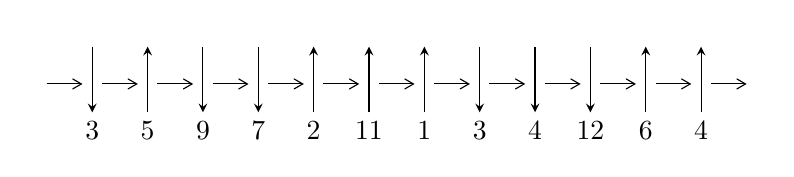
\begin{tikzpicture}[x=20pt, y=17pt]
	% nodes
	\node (C0) at (0, 0) {};
	\node (C1) at (1, 0) {};
	\node (C1U) at (1, +1) {};
	\node (C1D) at (1, -1) {3};

	\node (C2) at (2, 0) {};
	\node (C2U) at (2, +1) {};
	\node (C2D) at (2, -1) {5};

	\node (C3) at (3, 0) {};
	\node (C3U) at (3, +1) {};
	\node (C3D) at (3, -1) {9};

	\node (C4) at (4, 0) {};
	\node (C4U) at (4, +1) {};
	\node (C4D) at (4, -1) {7};

	\node (C5) at (5, 0) {};
	\node (C5U) at (5, +1) {};
	\node (C5D) at (5, -1) {2};

	\node (C6) at (6, 0) {};
	\node (C6U) at (6, +1) {};
	\node (C6D) at (6, -1) {11};

	\node (C7) at (7, 0) {};
	\node (C7U) at (7, +1) {};
	\node (C7D) at (7, -1) {1};

	\node (C8) at (8, 0) {};
	\node (C8U) at (8, +1) {};
	\node (C8D) at (8, -1) {3};

	\node (C9) at (9, 0) {};
	\node (C9U) at (9, +1) {};
	\node (C9D) at (9, -1) {4};

	\node (C10) at (10, 0) {};
	\node (C10U) at (10, +1) {};
	\node (C10D) at (10, -1) {12};

	\node (C11) at (11, 0) {};
	\node (C11U) at (11, +1) {};
	\node (C11D) at (11, -1) {6};

	\node (C12) at (12, 0) {};
	\node (C12U) at (12, +1) {};
	\node (C12D) at (12, -1) {4};
	\node (C13) at (13, 0) {};

	% arrows
	\draw[->,>={angle 60}]
	(C0) edge (C1) (C1) edge (C2) (C2) edge (C3) (C3) edge (C4) (C4) edge (C5) (C5) edge (C6) (C6) edge (C7) (C7) edge (C8) (C8) edge (C9) (C9) edge (C10) (C10) edge (C11) (C11) edge (C12) (C12) edge (C13) ;	\draw[->,>=stealth]
	(C1U) edge (C1D) (C2D) edge (C2U) (C3U) edge (C3D) (C4U) edge (C4D) (C5D) edge (C5U) (C6D) edge (C6U) (C7D) edge (C7U) (C8U) edge (C8D) (C9U) edge (C9D) (C10U) edge (C10D) (C11D) edge (C11U) (C12D) edge (C12U) ;
	\end{tikzpicture} \\
\hhline{~~} \\& 
\textbf{Solving Sequence} \\ \cline{2-2} 
 &
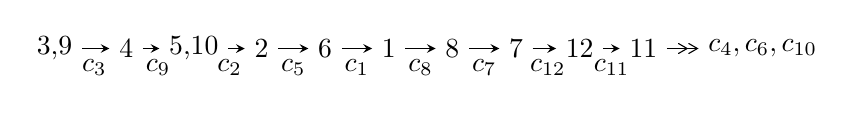
\begin{tikzpicture}[x=23pt, y=7pt]
	% node
	\node (A0) at (-1/8, 0) {3,9};
	\node (A1) at (1, 0) {4};
	\node (A2) at (33/16, 0) {5,10};
	\node (A3) at (25/8, 0) {2};
	\node (A4) at (33/8, 0) {6};
	\node (A5) at (41/8, 0) {1};
	\node (A6) at (49/8, 0) {8};
	\node (A7) at (57/8, 0) {7};
	\node (A8) at (65/8, 0) {12};
	\node (A9) at (73/8, 0) {11};
	\node (C1) at (1/2, -1) {$c_{3}$};
	\node (C2) at (3/2, -1) {$c_{9}$};
	\node (C3) at (21/8, -1) {$c_{2}$};
	\node (C4) at (29/8, -1) {$c_{5}$};
	\node (C5) at (37/8, -1) {$c_{1}$};
	\node (C6) at (45/8, -1) {$c_{8}$};
	\node (C7) at (53/8, -1) {$c_{7}$};
	\node (C8) at (61/8, -1) {$c_{12}$};
	\node (C9) at (69/8, -1) {$c_{11}$};
	\node (A10) at (11, 0) {$c_{4},c_{6},c_{10}$};

	% edge
	\draw[->,>=stealth]	
	(A0) edge (A1) (A1) edge (A2) (A2) edge (A3) (A3) edge (A4) (A4) edge (A5) (A5) edge (A6) (A6) edge (A7) (A7) edge (A8) (A8) edge (A9) ;
	\draw[->>,>={angle 60}]	
	(A9) edge (A10);
\end{tikzpicture} \\ 

\end{tabular} \\

\footnotetext{
The image of knot diagram is generated by the software ``\textbf{Draw programme}" developed by Andrew Bartholomew(\url{http://www.layer8.co.uk/maths/draw/index.htm\#Running-draw}), where we modified some parts for our purpose(\url{https://github.com/CATsTAILs/LinksPainter}).
}\phantom \\ \newline 
\centering \textbf{Ideals for irreducible components\footnotemark of $X_{\text{par}}$} 
 
\begin{align*}
I^u_{1}&=\langle 
- u^7+4 u^6-9 u^5+10 u^4-6 u^3+b- u+1,\;- u^7+4 u^6-9 u^5+10 u^4-7 u^3+u^2+a- u,\\
\phantom{I^u_{1}}&\phantom{= \langle  }u^8-5 u^7+13 u^6-19 u^5+17 u^4-8 u^3+3 u^2-2 u+1\rangle \\
I^u_{2}&=\langle 
- u^2 a- u^2+b,\;- u^7 a- u^6 a+u^7- u^5 a+u^6+u^4 a+u^5-2 u^3 a-2 u^4+u^3+a^2- u^2+a-1,\\
\phantom{I^u_{2}}&\phantom{= \langle  }u^8+2 u^7+3 u^6+u^5+2 u^4+u^3+2 u^2+u+1\rangle \\
I^u_{3}&=\langle 
- u^7+3 u^5-2 u^3+b- u+1,\;- u^7+3 u^5- u^3+u^2+a-3 u,\;u^8- u^7-3 u^6+3 u^5+u^4-2 u^3+3 u^2-2 u+1\rangle \\
I^u_{4}&=\langle 
5 u^7-17 u^6+17 u^5+28 u^4-71 u^3+8 u^2+8 b+112 u-104,\\
\phantom{I^u_{4}}&\phantom{= \langle  }17 u^7-57 u^6+61 u^5+92 u^4-231 u^3+36 u^2+32 a+356 u-344,\\
\phantom{I^u_{4}}&\phantom{= \langle  }u^8-5 u^7+9 u^6-23 u^4+24 u^3+20 u^2-56 u+32\rangle \\
I^u_{5}&=\langle 
2 u^{11}+5 u^{10}+5 u^9-2 u^8-7 u^7-8 u^6-9 u^5+3 u^4-4 u^2 a-2 u^3+7 u^2+4 b-7 u+1,\\
\phantom{I^u_{5}}&\phantom{= \langle  }6 u^{11} a-7 u^{11}+\cdots-9 a+25,\;u^{12}+3 u^{11}+4 u^{10}+u^9-3 u^8-5 u^7-6 u^6+3 u^3-3 u^2-2 u-1\rangle \\
I^u_{6}&=\langle 
- u^2 a- u^2+b,\;- u^3 a+u^3+a^2+2 a u+2 u^2+a- u-2,\;u^4+u^3- u^2- u-1\rangle \\
\\
\end{align*}
\raggedright * 6 irreducible components of $\dim_{\mathbb{C}}=0$, with total 72 representations.\\
\footnotetext{All coefficients of polynomials are rational numbers. But the coefficients are sometimes approximated in decimal forms when there is not enough margin.}
\newpage
\renewcommand{\arraystretch}{1}
\centering \section*{I. $I^u_{1}= \langle - u^7+4 u^6-9 u^5+10 u^4-6 u^3+b- u+1,\;- u^7+4 u^6-9 u^5+10 u^4-7 u^3+u^2+a- u,\;u^8-5 u^7+\cdots-2 u+1 \rangle$}
\flushleft \textbf{(i) Arc colorings}\\
\begin{tabular}{m{7pt} m{180pt} m{7pt} m{180pt} }
\flushright $a_{3}=$&$\begin{pmatrix}1\\0\end{pmatrix}$ \\
\flushright $a_{9}=$&$\begin{pmatrix}0\\u\end{pmatrix}$ \\
\flushright $a_{4}=$&$\begin{pmatrix}1\\u^2\end{pmatrix}$ \\
\flushright $a_{5}=$&$\begin{pmatrix}u^7-4 u^6+9 u^5-10 u^4+7 u^3- u^2+u\\u^7-4 u^6+9 u^5-10 u^4+6 u^3+u-1\end{pmatrix}$ \\
\flushright $a_{10}=$&$\begin{pmatrix}- u\\- u^3+u\end{pmatrix}$ \\
\flushright $a_{2}=$&$\begin{pmatrix}u^7-5 u^6+12 u^5-15 u^4+10 u^3-2 u^2+u-1\\u^5-3 u^4+4 u^3-2 u^2-1\end{pmatrix}$ \\
\flushright $a_{6}=$&$\begin{pmatrix}u^7-5 u^6+12 u^5-15 u^4+10 u^3-2 u^2+u-1\\- u^7+5 u^6-11 u^5+13 u^4-8 u^3+3 u^2-2 u+1\end{pmatrix}$ \\
\flushright $a_{1}=$&$\begin{pmatrix}u^7-5 u^6+13 u^5-18 u^4+14 u^3-4 u^2+u-2\\u^5-3 u^4+4 u^3-2 u^2-1\end{pmatrix}$ \\
\flushright $a_{8}=$&$\begin{pmatrix}u\\u\end{pmatrix}$ \\
\flushright $a_{7}=$&$\begin{pmatrix}u^7-4 u^6+9 u^5-10 u^4+7 u^3- u^2+2 u-1\\u^7-4 u^6+9 u^5-10 u^4+7 u^3-2 u^2+2 u-1\end{pmatrix}$ \\
\flushright $a_{12}=$&$\begin{pmatrix}u^7-4 u^6+9 u^5-11 u^4+8 u^3-2 u^2-1\\u^7-6 u^6+14 u^5-18 u^4+11 u^3-4 u^2+2 u-2\end{pmatrix}$ \\
\flushright $a_{11}=$&$\begin{pmatrix}u^7-5 u^6+12 u^5-16 u^4+11 u^3-3 u^2-2\\- u^6+3 u^5-5 u^4+4 u^3-2 u^2+u-1\end{pmatrix}$\\&\end{tabular}
\flushleft \textbf{(ii) Obstruction class $= -1$}\\~\\
\flushleft \textbf{(iii) Cusp Shapes $= 6 u^7-30 u^6+72 u^5-90 u^4+56 u^3-4 u^2-9$}\\~\\
\newpage\renewcommand{\arraystretch}{1}
\flushleft \textbf{(iv) u-Polynomials at the component}\newline \\
\begin{tabular}{m{50pt}|m{274pt}}
Crossings & \hspace{64pt}u-Polynomials at each crossing \\
\hline $$\begin{aligned}c_{1},c_{10}\end{aligned}$$&$\begin{aligned}
&u^8+3 u^7+8 u^6+15 u^5+19 u^4+24 u^3+18 u^2+4 u+1
\end{aligned}$\\
\hline $$\begin{aligned}c_{2},c_{5},c_{6}\\c_{11}\end{aligned}$$&$\begin{aligned}
&u^8+3 u^7+6 u^6+7 u^5+7 u^4+4 u^3+2 u^2+1
\end{aligned}$\\
\hline $$\begin{aligned}c_{3},c_{4},c_{8}\\c_{9}\end{aligned}$$&$\begin{aligned}
&u^8-5 u^7+13 u^6-19 u^5+17 u^4-8 u^3+3 u^2-2 u+1
\end{aligned}$\\
\hline $$\begin{aligned}c_{7},c_{12}\end{aligned}$$&$\begin{aligned}
&u^8+u^7-6 u^6-9 u^5+11 u^4+13 u^3+9 u^2+2 u+1
\end{aligned}$\\
\hline
\end{tabular}\\~\\
\newpage\renewcommand{\arraystretch}{1}
\flushleft \textbf{(v) Riley Polynomials at the component}\newline \\
\begin{tabular}{m{50pt}|m{274pt}}
Crossings & \hspace{64pt}Riley Polynomials at each crossing \\
\hline $$\begin{aligned}c_{1},c_{10}\end{aligned}$$&$\begin{aligned}
&y^8+7 y^7+12 y^6-29 y^5-93 y^4+4 y^3+170 y^2+20 y+1
\end{aligned}$\\
\hline $$\begin{aligned}c_{2},c_{5},c_{6}\\c_{11}\end{aligned}$$&$\begin{aligned}
&y^8+3 y^7+8 y^6+15 y^5+19 y^4+24 y^3+18 y^2+4 y+1
\end{aligned}$\\
\hline $$\begin{aligned}c_{3},c_{4},c_{8}\\c_{9}\end{aligned}$$&$\begin{aligned}
&y^8+y^7+13 y^6+7 y^5+45 y^4-12 y^3+11 y^2+2 y+1
\end{aligned}$\\
\hline $$\begin{aligned}c_{7},c_{12}\end{aligned}$$&$\begin{aligned}
&y^8-13 y^7+76 y^6-221 y^5+245 y^4+53 y^3+51 y^2+14 y+1
\end{aligned}$\\
\hline
\end{tabular}\\~\\
\newpage\flushleft \textbf{(vi) Complex Volumes and Cusp Shapes}
$$\begin{array}{c|c|c}  
\text{Solutions to }I^u_{1}& \I (\text{vol} + \sqrt{-1}CS) & \text{Cusp shape}\\
 \hline 
\begin{aligned}
u &= \phantom{-}0.652271 + 0.360769 I \\
a &= \phantom{-}0.732717 + 1.076160 I \\
b &= \phantom{-}0.005195 + 1.133280 I\end{aligned}
 & -4.98976 - 1.40911 I & -5.93719 + 4.96219 I \\ \hline\begin{aligned}
u &= \phantom{-}0.652271 - 0.360769 I \\
a &= \phantom{-}0.732717 - 1.076160 I \\
b &= \phantom{-}0.005195 - 1.133280 I\end{aligned}
 & -4.98976 + 1.40911 I & -5.93719 - 4.96219 I \\ \hline\begin{aligned}
u &= -0.260888 + 0.445572 I \\
a &= \phantom{-}0.965935 - 0.196423 I \\
b &= -0.302166 - 0.431430 I\end{aligned}
 & \phantom{-}0.040580 + 1.038860 I & \phantom{-}0.71134 - 6.68770 I \\ \hline\begin{aligned}
u &= -0.260888 - 0.445572 I \\
a &= \phantom{-}0.965935 + 0.196423 I \\
b &= -0.302166 + 0.431430 I\end{aligned}
 & \phantom{-}0.040580 - 1.038860 I & \phantom{-}0.71134 + 6.68770 I \\ \hline\begin{aligned}
u &= \phantom{-}0.89585 + 1.26725 I \\
a &= -0.831436 - 0.483431 I \\
b &= \phantom{-}0.962229 + 0.771104 I\end{aligned}
 & \phantom{-}10.00520 - 2.02473 I & \phantom{-}3.02254 - 0.14098 I \\ \hline\begin{aligned}
u &= \phantom{-}0.89585 - 1.26725 I \\
a &= -0.831436 + 0.483431 I \\
b &= \phantom{-}0.962229 - 0.771104 I\end{aligned}
 & \phantom{-}10.00520 + 2.02473 I & \phantom{-}3.02254 + 0.14098 I \\ \hline\begin{aligned}
u &= \phantom{-}1.21276 + 1.15424 I \\
a &= -1.367220 - 0.316333 I \\
b &= \phantom{-}0.834742 - 1.071900 I\end{aligned}
 & \phantom{-}8.1034 - 15.2709 I & \phantom{-}0.20330 + 8.45960 I \\ \hline\begin{aligned}
u &= \phantom{-}1.21276 - 1.15424 I \\
a &= -1.367220 + 0.316333 I \\
b &= \phantom{-}0.834742 + 1.071900 I\end{aligned}
 & \phantom{-}8.1034 + 15.2709 I & \phantom{-}0.20330 - 8.45960 I\\
 \hline 
 \end{array}$$\newpage\newpage\renewcommand{\arraystretch}{1}
\centering \section*{II. $I^u_{2}= \langle - u^2 a- u^2+b,\;- u^7 a+u^7+\cdots+a-1,\;u^8+2 u^7+3 u^6+u^5+2 u^4+u^3+2 u^2+u+1 \rangle$}
\flushleft \textbf{(i) Arc colorings}\\
\begin{tabular}{m{7pt} m{180pt} m{7pt} m{180pt} }
\flushright $a_{3}=$&$\begin{pmatrix}1\\0\end{pmatrix}$ \\
\flushright $a_{9}=$&$\begin{pmatrix}0\\u\end{pmatrix}$ \\
\flushright $a_{4}=$&$\begin{pmatrix}1\\u^2\end{pmatrix}$ \\
\flushright $a_{5}=$&$\begin{pmatrix}a\\u^2 a+u^2\end{pmatrix}$ \\
\flushright $a_{10}=$&$\begin{pmatrix}- u\\- u^3+u\end{pmatrix}$ \\
\flushright $a_{2}=$&$\begin{pmatrix}u^6 a+u^5 a+u^4 a- u^3 a+u^2 a+u^3+a\\- u^7 a-2 u^6 a-2 u^5 a+u^5- u^3 a+u^4- u^2 a- a u- u^2- a\end{pmatrix}$ \\
\flushright $a_{6}=$&$\begin{pmatrix}u^6 a+u^5 a+u^4 a- u^3 a+u^2 a+u^3+a\\- u^6 a+u^7- u^5 a+u^6-2 u^4 a+u^5-2 u^4- u^2 a+u^2- a\end{pmatrix}$ \\
\flushright $a_{1}=$&$\begin{pmatrix}- u^7 a- u^6 a- u^5 a+u^4 a+u^5-2 u^3 a+u^4+u^3- a u- u^2\\- u^7 a-2 u^6 a-2 u^5 a+u^5- u^3 a+u^4- u^2 a- a u- u^2- a\end{pmatrix}$ \\
\flushright $a_{8}=$&$\begin{pmatrix}u\\u\end{pmatrix}$ \\
\flushright $a_{7}=$&$\begin{pmatrix}- u^7 a+u^7+\cdots- a+1\\a u\end{pmatrix}$ \\
\flushright $a_{12}=$&$\begin{pmatrix}u^7+u^6+u^5- u^3 a- u^4+u^3\\- u^7 a- u^6 a- u^7-2 u^5 a+u^4 a- u^3 a+3 u^4- u^3- a u+1\end{pmatrix}$ \\
\flushright $a_{11}=$&$\begin{pmatrix}- u^7 a+u^7+\cdots- a+1\\-2 u^7-3 u^6-4 u^5+u^3 a-3 u^3-2 u^2-3 u-1\end{pmatrix}$\\&\end{tabular}
\flushleft \textbf{(ii) Obstruction class $= -1$}\\~\\
\flushleft \textbf{(iii) Cusp Shapes $= -7 u^7-9 u^6-8 u^5+13 u^4-2 u^3+4 u^2-5 u+4$}\\~\\
\newpage\renewcommand{\arraystretch}{1}
\flushleft \textbf{(iv) u-Polynomials at the component}\newline \\
\begin{tabular}{m{50pt}|m{274pt}}
Crossings & \hspace{64pt}u-Polynomials at each crossing \\
\hline $$\begin{aligned}c_{1},c_{10}\end{aligned}$$&$\begin{aligned}
&u^{16}+4 u^{15}+\cdots+128 u+256
\end{aligned}$\\
\hline $$\begin{aligned}c_{2},c_{5},c_{6}\\c_{11}\end{aligned}$$&$\begin{aligned}
&u^{16}+4 u^{15}+\cdots+48 u+16
\end{aligned}$\\
\hline $$\begin{aligned}c_{3},c_{4},c_{8}\\c_{9}\end{aligned}$$&$\begin{aligned}
&(u^8+2 u^7+3 u^6+u^5+2 u^4+u^3+2 u^2+u+1)^2
\end{aligned}$\\
\hline $$\begin{aligned}c_{7},c_{12}\end{aligned}$$&$\begin{aligned}
&u^{16}+2 u^{15}+\cdots+2 u+1
\end{aligned}$\\
\hline
\end{tabular}\\~\\
\newpage\renewcommand{\arraystretch}{1}
\flushleft \textbf{(v) Riley Polynomials at the component}\newline \\
\begin{tabular}{m{50pt}|m{274pt}}
Crossings & \hspace{64pt}Riley Polynomials at each crossing \\
\hline $$\begin{aligned}c_{1},c_{10}\end{aligned}$$&$\begin{aligned}
&y^{16}+12 y^{15}+\cdots+237568 y+65536
\end{aligned}$\\
\hline $$\begin{aligned}c_{2},c_{5},c_{6}\\c_{11}\end{aligned}$$&$\begin{aligned}
&y^{16}+4 y^{15}+\cdots+128 y+256
\end{aligned}$\\
\hline $$\begin{aligned}c_{3},c_{4},c_{8}\\c_{9}\end{aligned}$$&$\begin{aligned}
&(y^8+2 y^7+9 y^6+11 y^5+12 y^4+11 y^3+6 y^2+3 y+1)^2
\end{aligned}$\\
\hline $$\begin{aligned}c_{7},c_{12}\end{aligned}$$&$\begin{aligned}
&y^{16}-34 y^{15}+\cdots+34 y+1
\end{aligned}$\\
\hline
\end{tabular}\\~\\
\newpage\flushleft \textbf{(vi) Complex Volumes and Cusp Shapes}
$$\begin{array}{c|c|c}  
\text{Solutions to }I^u_{2}& \I (\text{vol} + \sqrt{-1}CS) & \text{Cusp shape}\\
 \hline 
\begin{aligned}
u &= \phantom{-}0.669857 + 0.618731 I \\
a &= \phantom{-}0.519643 + 0.618737 I \\
b &= -0.412772 + 1.300430 I\end{aligned}
 & -0.68359 - 8.02114 I & -3.38988 + 11.48011 I \\ \hline\begin{aligned}
u &= \phantom{-}0.669857 + 0.618731 I \\
a &= -2.17987 - 0.90212 I \\
b &= \phantom{-}0.670058 - 1.037450 I\end{aligned}
 & -0.68359 - 8.02114 I & -3.38988 + 11.48011 I \\ \hline\begin{aligned}
u &= \phantom{-}0.669857 - 0.618731 I \\
a &= \phantom{-}0.519643 - 0.618737 I \\
b &= -0.412772 - 1.300430 I\end{aligned}
 & -0.68359 + 8.02114 I & -3.38988 - 11.48011 I \\ \hline\begin{aligned}
u &= \phantom{-}0.669857 - 0.618731 I \\
a &= -2.17987 + 0.90212 I \\
b &= \phantom{-}0.670058 + 1.037450 I\end{aligned}
 & -0.68359 + 8.02114 I & -3.38988 - 11.48011 I \\ \hline\begin{aligned}
u &= -0.575075 + 0.604029 I \\
a &= -0.206518 + 1.127330 I \\
b &= \phantom{-}0.756093 - 0.589737 I\end{aligned}
 & \phantom{-}0.63668 + 2.58489 I & -1.22299 - 5.26005 I \\ \hline\begin{aligned}
u &= -0.575075 + 0.604029 I \\
a &= \phantom{-}0.634679 - 0.563795 I \\
b &= -0.447489 - 1.116400 I\end{aligned}
 & \phantom{-}0.63668 + 2.58489 I & -1.22299 - 5.26005 I \\ \hline\begin{aligned}
u &= -0.575075 - 0.604029 I \\
a &= -0.206518 - 1.127330 I \\
b &= \phantom{-}0.756093 + 0.589737 I\end{aligned}
 & \phantom{-}0.63668 - 2.58489 I & -1.22299 + 5.26005 I \\ \hline\begin{aligned}
u &= -0.575075 - 0.604029 I \\
a &= \phantom{-}0.634679 + 0.563795 I \\
b &= -0.447489 + 1.116400 I\end{aligned}
 & \phantom{-}0.63668 - 2.58489 I & -1.22299 + 5.26005 I \\ \hline\begin{aligned}
u &= -0.046597 + 0.820905 I \\
a &= \phantom{-}0.633387 - 0.032164 I \\
b &= -1.099630 - 0.103355 I\end{aligned}
 & \phantom{-}4.09203 + 2.71750 I & \phantom{-}9.92245 - 2.29698 I \\ \hline\begin{aligned}
u &= -0.046597 + 0.820905 I \\
a &= -2.18872 - 1.14293 I \\
b &= \phantom{-}0.711041 + 0.858664 I\end{aligned}
 & \phantom{-}4.09203 + 2.71750 I & \phantom{-}9.92245 - 2.29698 I\\
 \hline 
 \end{array}$$\newpage$$\begin{array}{c|c|c}  
\text{Solutions to }I^u_{2}& \I (\text{vol} + \sqrt{-1}CS) & \text{Cusp shape}\\
 \hline 
\begin{aligned}
u &= -0.046597 - 0.820905 I \\
a &= \phantom{-}0.633387 + 0.032164 I \\
b &= -1.099630 + 0.103355 I\end{aligned}
 & \phantom{-}4.09203 - 2.71750 I & \phantom{-}9.92245 + 2.29698 I \\ \hline\begin{aligned}
u &= -0.046597 - 0.820905 I \\
a &= -2.18872 + 1.14293 I \\
b &= \phantom{-}0.711041 - 0.858664 I\end{aligned}
 & \phantom{-}4.09203 - 2.71750 I & \phantom{-}9.92245 + 2.29698 I \\ \hline\begin{aligned}
u &= -1.04818 + 1.20777 I \\
a &= -0.761541 + 0.428484 I \\
b &= \phantom{-}0.999043 - 0.758029 I\end{aligned}
 & \phantom{-}9.11436 + 8.57751 I & \phantom{-}1.69041 - 4.42296 I \\ \hline\begin{aligned}
u &= -1.04818 + 1.20777 I \\
a &= -1.45106 + 0.26117 I \\
b &= \phantom{-}0.823655 + 1.048040 I\end{aligned}
 & \phantom{-}9.11436 + 8.57751 I & \phantom{-}1.69041 - 4.42296 I \\ \hline\begin{aligned}
u &= -1.04818 - 1.20777 I \\
a &= -0.761541 - 0.428484 I \\
b &= \phantom{-}0.999043 + 0.758029 I\end{aligned}
 & \phantom{-}9.11436 - 8.57751 I & \phantom{-}1.69041 + 4.42296 I \\ \hline\begin{aligned}
u &= -1.04818 - 1.20777 I \\
a &= -1.45106 - 0.26117 I \\
b &= \phantom{-}0.823655 - 1.048040 I\end{aligned}
 & \phantom{-}9.11436 - 8.57751 I & \phantom{-}1.69041 + 4.42296 I\\
 \hline 
 \end{array}$$\newpage\newpage\renewcommand{\arraystretch}{1}
\centering \section*{III. $I^u_{3}= \langle - u^7+3 u^5-2 u^3+b- u+1,\;- u^7+3 u^5- u^3+u^2+a-3 u,\;u^8- u^7-3 u^6+3 u^5+u^4-2 u^3+3 u^2-2 u+1 \rangle$}
\flushleft \textbf{(i) Arc colorings}\\
\begin{tabular}{m{7pt} m{180pt} m{7pt} m{180pt} }
\flushright $a_{3}=$&$\begin{pmatrix}1\\0\end{pmatrix}$ \\
\flushright $a_{9}=$&$\begin{pmatrix}0\\u\end{pmatrix}$ \\
\flushright $a_{4}=$&$\begin{pmatrix}1\\u^2\end{pmatrix}$ \\
\flushright $a_{5}=$&$\begin{pmatrix}u^7-3 u^5+u^3- u^2+3 u\\u^7-3 u^5+2 u^3+u-1\end{pmatrix}$ \\
\flushright $a_{10}=$&$\begin{pmatrix}- u\\- u^3+u\end{pmatrix}$ \\
\flushright $a_{2}=$&$\begin{pmatrix}u^7- u^6-4 u^5+3 u^4+4 u^3-2 u^2+u-1\\u^5+u^4-2 u^3-2 u^2-1\end{pmatrix}$ \\
\flushright $a_{6}=$&$\begin{pmatrix}- u^7+u^6+4 u^5-3 u^4-4 u^3+2 u^2- u+1\\u^7+u^6-3 u^5-3 u^4+2 u^3+u^2+1\end{pmatrix}$ \\
\flushright $a_{1}=$&$\begin{pmatrix}u^7- u^6-3 u^5+4 u^4+2 u^3-4 u^2+u-2\\u^5+u^4-2 u^3-2 u^2-1\end{pmatrix}$ \\
\flushright $a_{8}=$&$\begin{pmatrix}u\\u\end{pmatrix}$ \\
\flushright $a_{7}=$&$\begin{pmatrix}- u^7+3 u^5- u^3+u^2-2 u-1\\- u^7+3 u^5- u^3-2 u+1\end{pmatrix}$ \\
\flushright $a_{12}=$&$\begin{pmatrix}u^7-3 u^5+u^4+2 u^3-2 u^2-1\\u^7-2 u^5+2 u^4- u^3-4 u^2+2 u-2\end{pmatrix}$ \\
\flushright $a_{11}=$&$\begin{pmatrix}- u^7+u^6+4 u^5-2 u^4-3 u^3+u^2-4 u\\u^6+u^5- u^4-2 u^3-2 u^2- u+1\end{pmatrix}$\\&\end{tabular}
\flushleft \textbf{(ii) Obstruction class $= 1$}\\~\\
\flushleft \textbf{(iii) Cusp Shapes $= 2 u^7-2 u^6-12 u^5+2 u^4+16 u^3+4 u+3$}\\~\\
\newpage\renewcommand{\arraystretch}{1}
\flushleft \textbf{(iv) u-Polynomials at the component}\newline \\
\begin{tabular}{m{50pt}|m{274pt}}
Crossings & \hspace{64pt}u-Polynomials at each crossing \\
\hline $$\begin{aligned}c_{1},c_{10}\end{aligned}$$&$\begin{aligned}
&u^8-3 u^7+8 u^6-11 u^5+15 u^4-12 u^3+10 u^2-4 u+1
\end{aligned}$\\
\hline $$\begin{aligned}c_{2},c_{6}\end{aligned}$$&$\begin{aligned}
&u^8+u^7+2 u^6+u^5+3 u^4+2 u^3+2 u^2+1
\end{aligned}$\\
\hline $$\begin{aligned}c_{3}\end{aligned}$$&$\begin{aligned}
&u^8- u^7-3 u^6+3 u^5+u^4-2 u^3+3 u^2-2 u+1
\end{aligned}$\\
\hline $$\begin{aligned}c_{4},c_{8},c_{9}\end{aligned}$$&$\begin{aligned}
&u^8+u^7-3 u^6-3 u^5+u^4+2 u^3+3 u^2+2 u+1
\end{aligned}$\\
\hline $$\begin{aligned}c_{5},c_{11}\end{aligned}$$&$\begin{aligned}
&u^8- u^7+2 u^6- u^5+3 u^4-2 u^3+2 u^2+1
\end{aligned}$\\
\hline $$\begin{aligned}c_{7},c_{12}\end{aligned}$$&$\begin{aligned}
&u^8- u^7- u^5+3 u^4-3 u^3+u^2+1
\end{aligned}$\\
\hline
\end{tabular}\\~\\
\newpage\renewcommand{\arraystretch}{1}
\flushleft \textbf{(v) Riley Polynomials at the component}\newline \\
\begin{tabular}{m{50pt}|m{274pt}}
Crossings & \hspace{64pt}Riley Polynomials at each crossing \\
\hline $$\begin{aligned}c_{1},c_{10}\end{aligned}$$&$\begin{aligned}
&y^8+7 y^7+28 y^6+67 y^5+99 y^4+84 y^3+34 y^2+4 y+1
\end{aligned}$\\
\hline $$\begin{aligned}c_{2},c_{5},c_{6}\\c_{11}\end{aligned}$$&$\begin{aligned}
&y^8+3 y^7+8 y^6+11 y^5+15 y^4+12 y^3+10 y^2+4 y+1
\end{aligned}$\\
\hline $$\begin{aligned}c_{3},c_{4},c_{8}\\c_{9}\end{aligned}$$&$\begin{aligned}
&y^8-7 y^7+17 y^6-13 y^5-7 y^4+8 y^3+3 y^2+2 y+1
\end{aligned}$\\
\hline $$\begin{aligned}c_{7},c_{12}\end{aligned}$$&$\begin{aligned}
&y^8- y^7+4 y^6-5 y^5+5 y^4-3 y^3+7 y^2+2 y+1
\end{aligned}$\\
\hline
\end{tabular}\\~\\
\newpage\flushleft \textbf{(vi) Complex Volumes and Cusp Shapes}
$$\begin{array}{c|c|c}  
\text{Solutions to }I^u_{3}& \I (\text{vol} + \sqrt{-1}CS) & \text{Cusp shape}\\
 \hline 
\begin{aligned}
u &= -0.030890 + 0.718197 I \\
a &= \phantom{-}0.622175 + 1.173170 I \\
b &= -0.783128 - 0.675988 I\end{aligned}
 & \phantom{-}3.07236 + 3.68820 I & \phantom{-}4.98393 - 5.29986 I \\ \hline\begin{aligned}
u &= -0.030890 - 0.718197 I \\
a &= \phantom{-}0.622175 - 1.173170 I \\
b &= -0.783128 + 0.675988 I\end{aligned}
 & \phantom{-}3.07236 - 3.68820 I & \phantom{-}4.98393 + 5.29986 I \\ \hline\begin{aligned}
u &= \phantom{-}0.472052 + 0.470170 I \\
a &= \phantom{-}1.52839 + 1.41091 I \\
b &= -0.621805 + 1.124830 I\end{aligned}
 & \phantom{-}0.10782 - 7.15810 I & \phantom{-}2.37662 + 6.44391 I \\ \hline\begin{aligned}
u &= \phantom{-}0.472052 - 0.470170 I \\
a &= \phantom{-}1.52839 - 1.41091 I \\
b &= -0.621805 - 1.124830 I\end{aligned}
 & \phantom{-}0.10782 + 7.15810 I & \phantom{-}2.37662 - 6.44391 I \\ \hline\begin{aligned}
u &= -1.40119 + 0.27682 I \\
a &= -0.990196 + 0.324197 I \\
b &= \phantom{-}0.269993 + 0.604062 I\end{aligned}
 & -5.44591 + 2.04290 I & -7.10763 + 1.33066 I \\ \hline\begin{aligned}
u &= -1.40119 - 0.27682 I \\
a &= -0.990196 - 0.324197 I \\
b &= \phantom{-}0.269993 - 0.604062 I\end{aligned}
 & -5.44591 - 2.04290 I & -7.10763 - 1.33066 I \\ \hline\begin{aligned}
u &= \phantom{-}1.46003 + 0.07298 I \\
a &= -0.660372 + 0.409353 I \\
b &= \phantom{-}0.634940 + 0.942808 I\end{aligned}
 & -4.31401 + 5.00304 I & -2.25292 - 6.22083 I \\ \hline\begin{aligned}
u &= \phantom{-}1.46003 - 0.07298 I \\
a &= -0.660372 - 0.409353 I \\
b &= \phantom{-}0.634940 - 0.942808 I\end{aligned}
 & -4.31401 - 5.00304 I & -2.25292 + 6.22083 I\\
 \hline 
 \end{array}$$\newpage\newpage\renewcommand{\arraystretch}{1}
\centering \section*{IV. $I^u_{4}= \langle 5 u^7-17 u^6+\cdots+8 b-104,\;17 u^7-57 u^6+\cdots+32 a-344,\;u^8-5 u^7+\cdots-56 u+32 \rangle$}
\flushleft \textbf{(i) Arc colorings}\\
\begin{tabular}{m{7pt} m{180pt} m{7pt} m{180pt} }
\flushright $a_{3}=$&$\begin{pmatrix}1\\0\end{pmatrix}$ \\
\flushright $a_{9}=$&$\begin{pmatrix}0\\u\end{pmatrix}$ \\
\flushright $a_{4}=$&$\begin{pmatrix}1\\u^2\end{pmatrix}$ \\
\flushright $a_{5}=$&$\begin{pmatrix}-0.531250 u^{7}+1.78125 u^{6}+\cdots-11.1250 u+10.7500\\-\frac{5}{8} u^7+\frac{17}{8} u^6+\cdots-14 u+13\end{pmatrix}$ \\
\flushright $a_{10}=$&$\begin{pmatrix}- u\\- u^3+u\end{pmatrix}$ \\
\flushright $a_{2}=$&$\begin{pmatrix}\frac{1}{32} u^7-\frac{9}{32} u^6+\cdots+\frac{19}{8} u-\frac{13}{4}\\-\frac{3}{8} u^7+\frac{13}{8} u^6+\cdots-\frac{23}{2} u+11\end{pmatrix}$ \\
\flushright $a_{6}=$&$\begin{pmatrix}-\frac{1}{2} u^7+\frac{15}{8} u^6+\cdots-13 u+\frac{27}{2}\\-\frac{3}{8} u^7+\frac{7}{8} u^6+\cdots-\frac{9}{2} u+4\end{pmatrix}$ \\
\flushright $a_{1}=$&$\begin{pmatrix}-0.343750 u^{7}+1.34375 u^{6}+\cdots-9.12500 u+7.75000\\-\frac{3}{8} u^7+\frac{13}{8} u^6+\cdots-\frac{23}{2} u+11\end{pmatrix}$ \\
\flushright $a_{8}=$&$\begin{pmatrix}u\\u\end{pmatrix}$ \\
\flushright $a_{7}=$&$\begin{pmatrix}\frac{1}{32} u^7-\frac{1}{32} u^6+\cdots+\frac{7}{8} u+\frac{1}{4}\\\frac{1}{8} u^7-\frac{3}{8} u^6+\cdots+3 u-1\end{pmatrix}$ \\
\flushright $a_{12}=$&$\begin{pmatrix}-0.218750 u^{7}+0.968750 u^{6}+\cdots-7.62500 u+8.75000\\-\frac{3}{8} u^7+\frac{5}{8} u^6+\cdots-\frac{3}{2} u+3\end{pmatrix}$ \\
\flushright $a_{11}=$&$\begin{pmatrix}-0.218750 u^{7}+0.718750 u^{6}+\cdots-5.12500 u+4.25000\\-\frac{5}{8} u^7+\frac{15}{8} u^6+\cdots-11 u+11\end{pmatrix}$\\&\end{tabular}
\flushleft \textbf{(ii) Obstruction class $= -1$}\\~\\
\flushleft \textbf{(iii) Cusp Shapes $= 8 u^7-30 u^6+34 u^5+46 u^4-132 u^3+26 u^2+204 u-198$}\\~\\
\newpage\renewcommand{\arraystretch}{1}
\flushleft \textbf{(iv) u-Polynomials at the component}\newline \\
\begin{tabular}{m{50pt}|m{274pt}}
Crossings & \hspace{64pt}u-Polynomials at each crossing \\
\hline $$\begin{aligned}c_{1},c_{10}\end{aligned}$$&$\begin{aligned}
&(u^4+u^3+3 u^2+2 u+1)^2
\end{aligned}$\\
\hline $$\begin{aligned}c_{2},c_{5},c_{6}\\c_{11}\end{aligned}$$&$\begin{aligned}
&(u^4- u^3+u^2+1)^2
\end{aligned}$\\
\hline $$\begin{aligned}c_{3},c_{4},c_{8}\\c_{9}\end{aligned}$$&$\begin{aligned}
&u^8-5 u^7+9 u^6-23 u^4+24 u^3+20 u^2-56 u+32
\end{aligned}$\\
\hline $$\begin{aligned}c_{7},c_{12}\end{aligned}$$&$\begin{aligned}
&u^8-5 u^6-7 u^5+3 u^4+20 u^3+23 u^2-5 u+2
\end{aligned}$\\
\hline
\end{tabular}\\~\\
\newpage\renewcommand{\arraystretch}{1}
\flushleft \textbf{(v) Riley Polynomials at the component}\newline \\
\begin{tabular}{m{50pt}|m{274pt}}
Crossings & \hspace{64pt}Riley Polynomials at each crossing \\
\hline $$\begin{aligned}c_{1},c_{10}\end{aligned}$$&$\begin{aligned}
&(y^4+5 y^3+7 y^2+2 y+1)^2
\end{aligned}$\\
\hline $$\begin{aligned}c_{2},c_{5},c_{6}\\c_{11}\end{aligned}$$&$\begin{aligned}
&(y^4+y^3+3 y^2+2 y+1)^2
\end{aligned}$\\
\hline $$\begin{aligned}c_{3},c_{4},c_{8}\\c_{9}\end{aligned}$$&$\begin{aligned}
&y^8-7 y^7+\cdots-1856 y+1024
\end{aligned}$\\
\hline $$\begin{aligned}c_{7},c_{12}\end{aligned}$$&$\begin{aligned}
&y^8-10 y^7+31 y^6-33 y^5+63 y^4-352 y^3+741 y^2+67 y+4
\end{aligned}$\\
\hline
\end{tabular}\\~\\
\newpage\flushleft \textbf{(vi) Complex Volumes and Cusp Shapes}
$$\begin{array}{c|c|c}  
\text{Solutions to }I^u_{4}& \I (\text{vol} + \sqrt{-1}CS) & \text{Cusp shape}\\
 \hline 
\begin{aligned}
u &= -1.307400 + 0.487823 I \\
a &= -0.954979 - 0.171241 I \\
b &= \phantom{-}0.351808 + 0.720342 I\end{aligned}
 & -5.35681 + 2.83021 I & -5.65348 - 9.81749 I \\ \hline\begin{aligned}
u &= -1.307400 - 0.487823 I \\
a &= -0.954979 + 0.171241 I \\
b &= \phantom{-}0.351808 - 0.720342 I\end{aligned}
 & -5.35681 - 2.83021 I & -5.65348 + 9.81749 I \\ \hline\begin{aligned}
u &= \phantom{-}1.408170 + 0.087291 I \\
a &= -0.681944 - 0.925546 I \\
b &= \phantom{-}0.351808 - 0.720342 I\end{aligned}
 & -5.35681 - 2.83021 I & -5.65348 + 9.81749 I \\ \hline\begin{aligned}
u &= \phantom{-}1.408170 - 0.087291 I \\
a &= -0.681944 + 0.925546 I \\
b &= \phantom{-}0.351808 + 0.720342 I\end{aligned}
 & -5.35681 + 2.83021 I & -5.65348 - 9.81749 I \\ \hline\begin{aligned}
u &= \phantom{-}1.30983 + 1.01957 I \\
a &= \phantom{-}1.331510 + 0.422810 I \\
b &= -0.851808 + 0.911292 I\end{aligned}
 & \phantom{-}8.64668 - 6.32793 I & \phantom{-}1.65348 + 5.12960 I \\ \hline\begin{aligned}
u &= \phantom{-}1.30983 - 1.01957 I \\
a &= \phantom{-}1.331510 - 0.422810 I \\
b &= -0.851808 - 0.911292 I\end{aligned}
 & \phantom{-}8.64668 + 6.32793 I & \phantom{-}1.65348 - 5.12960 I \\ \hline\begin{aligned}
u &= \phantom{-}1.08940 + 1.34521 I \\
a &= \phantom{-}0.680418 + 0.376735 I \\
b &= -0.851808 - 0.911292 I\end{aligned}
 & \phantom{-}8.64668 + 6.32793 I & \phantom{-}1.65348 - 5.12960 I \\ \hline\begin{aligned}
u &= \phantom{-}1.08940 - 1.34521 I \\
a &= \phantom{-}0.680418 - 0.376735 I \\
b &= -0.851808 + 0.911292 I\end{aligned}
 & \phantom{-}8.64668 - 6.32793 I & \phantom{-}1.65348 + 5.12960 I\\
 \hline 
 \end{array}$$\newpage\newpage\renewcommand{\arraystretch}{1}
\centering \section*{V. $I^u_{5}= \langle 2 u^{11}+5 u^{10}+\cdots+4 b+1,\;6 u^{11} a-7 u^{11}+\cdots-9 a+25,\;u^{12}+3 u^{11}+\cdots-2 u-1 \rangle$}
\flushleft \textbf{(i) Arc colorings}\\
\begin{tabular}{m{7pt} m{180pt} m{7pt} m{180pt} }
\flushright $a_{3}=$&$\begin{pmatrix}1\\0\end{pmatrix}$ \\
\flushright $a_{9}=$&$\begin{pmatrix}0\\u\end{pmatrix}$ \\
\flushright $a_{4}=$&$\begin{pmatrix}1\\u^2\end{pmatrix}$ \\
\flushright $a_{5}=$&$\begin{pmatrix}a\\-\frac{1}{2} u^{11}-\frac{5}{4} u^{10}+\cdots+\frac{7}{4} u-\frac{1}{4}\end{pmatrix}$ \\
\flushright $a_{10}=$&$\begin{pmatrix}- u\\- u^3+u\end{pmatrix}$ \\
\flushright $a_{2}=$&$\begin{pmatrix}-\frac{1}{2} u^{11} a-\frac{3}{4} u^{11}+\cdots+\frac{1}{2} a+1\\-\frac{1}{4} u^{10} a+\frac{3}{4} u^{11}+\cdots+\frac{1}{2} a-1\end{pmatrix}$ \\
\flushright $a_{6}=$&$\begin{pmatrix}-\frac{1}{4} u^{10} a+\frac{1}{2} u^{11}+\cdots+a-\frac{11}{4}\\\frac{1}{4} u^{10} a-\frac{5}{4} u^{11}+\cdots-\frac{1}{4} a+\frac{3}{2}\end{pmatrix}$ \\
\flushright $a_{1}=$&$\begin{pmatrix}-\frac{1}{2} u^{11} a-\frac{3}{2} u^{10} a+\cdots+a-\frac{3}{4} u\\-\frac{1}{4} u^{10} a+\frac{3}{4} u^{11}+\cdots+\frac{1}{2} a-1\end{pmatrix}$ \\
\flushright $a_{8}=$&$\begin{pmatrix}u\\u\end{pmatrix}$ \\
\flushright $a_{7}=$&$\begin{pmatrix}-\frac{1}{4} u^{11} a+\frac{1}{4} u^{11}+\cdots+\frac{7}{4} a u-\frac{7}{4} u\\\frac{1}{2} u^{11}+\frac{3}{2} u^{10}+\cdots-\frac{7}{4} u-1\end{pmatrix}$ \\
\flushright $a_{12}=$&$\begin{pmatrix}-\frac{1}{4} u^{11} a- u^{11}+\cdots+\frac{1}{2} a+1\\-\frac{1}{4} u^{11} a+u^{11}+\cdots+\frac{1}{2} a-\frac{3}{4}\end{pmatrix}$ \\
\flushright $a_{11}=$&$\begin{pmatrix}-\frac{1}{4} u^{11} a+\frac{1}{4} u^{11}+\cdots+\frac{3}{2} a u-3 u\\-\frac{1}{4} u^{11} a+\frac{3}{4} u^{11}+\cdots-\frac{1}{2} u-1\end{pmatrix}$\\&\end{tabular}
\flushleft \textbf{(ii) Obstruction class $= -1$}\\~\\
\flushleft \textbf{(iii) Cusp Shapes $= u^{11}+2 u^{10}+u^9-3 u^8-5 u^7-5 u^6-4 u^5+7 u^4+5 u^3+6 u^2-4 u-3$}\\~\\
\newpage\renewcommand{\arraystretch}{1}
\flushleft \textbf{(iv) u-Polynomials at the component}\newline \\
\begin{tabular}{m{50pt}|m{274pt}}
Crossings & \hspace{64pt}u-Polynomials at each crossing \\
\hline $$\begin{aligned}c_{1},c_{10}\end{aligned}$$&$\begin{aligned}
&(u^4+u^3+3 u^2+2 u+1)^6
\end{aligned}$\\
\hline $$\begin{aligned}c_{2},c_{5},c_{6}\\c_{11}\end{aligned}$$&$\begin{aligned}
&(u^4- u^3+u^2+1)^6
\end{aligned}$\\
\hline $$\begin{aligned}c_{3},c_{4},c_{8}\\c_{9}\end{aligned}$$&$\begin{aligned}
&(u^{12}+3 u^{11}+4 u^{10}+u^9-3 u^8-5 u^7-6 u^6+3 u^3-3 u^2-2 u-1)^2
\end{aligned}$\\
\hline $$\begin{aligned}c_{7},c_{12}\end{aligned}$$&$\begin{aligned}
&u^{24}+3 u^{23}+\cdots+2368 u+1016
\end{aligned}$\\
\hline
\end{tabular}\\~\\
\newpage\renewcommand{\arraystretch}{1}
\flushleft \textbf{(v) Riley Polynomials at the component}\newline \\
\begin{tabular}{m{50pt}|m{274pt}}
Crossings & \hspace{64pt}Riley Polynomials at each crossing \\
\hline $$\begin{aligned}c_{1},c_{10}\end{aligned}$$&$\begin{aligned}
&(y^4+5 y^3+7 y^2+2 y+1)^6
\end{aligned}$\\
\hline $$\begin{aligned}c_{2},c_{5},c_{6}\\c_{11}\end{aligned}$$&$\begin{aligned}
&(y^4+y^3+3 y^2+2 y+1)^6
\end{aligned}$\\
\hline $$\begin{aligned}c_{3},c_{4},c_{8}\\c_{9}\end{aligned}$$&$\begin{aligned}
&(y^{12}- y^{11}+\cdots+2 y+1)^{2}
\end{aligned}$\\
\hline $$\begin{aligned}c_{7},c_{12}\end{aligned}$$&$\begin{aligned}
&y^{24}-3 y^{23}+\cdots-1653152 y+1032256
\end{aligned}$\\
\hline
\end{tabular}\\~\\
\newpage\flushleft \textbf{(vi) Complex Volumes and Cusp Shapes}
$$\begin{array}{c|c|c}  
\text{Solutions to }I^u_{5}& \I (\text{vol} + \sqrt{-1}CS) & \text{Cusp shape}\\
 \hline 
\begin{aligned}
u &= -0.535167 + 0.929438 I \\
a &= \phantom{-}0.528827 + 0.711224 I \\
b &= \phantom{-}0.351808 - 0.720342 I\end{aligned}
 & \phantom{-}1.64493 + 1.74886 I & -2.00000 + 2.34394 I \\ \hline\begin{aligned}
u &= -0.535167 + 0.929438 I \\
a &= \phantom{-}1.197710 - 0.110412 I \\
b &= -0.851808 - 0.911292 I\end{aligned}
 & \phantom{-}1.64493 + 1.74886 I & -2.00000 + 2.34394 I \\ \hline\begin{aligned}
u &= -0.535167 - 0.929438 I \\
a &= \phantom{-}0.528827 - 0.711224 I \\
b &= \phantom{-}0.351808 + 0.720342 I\end{aligned}
 & \phantom{-}1.64493 - 1.74886 I & -2.00000 - 2.34394 I \\ \hline\begin{aligned}
u &= -0.535167 - 0.929438 I \\
a &= \phantom{-}1.197710 + 0.110412 I \\
b &= -0.851808 + 0.911292 I\end{aligned}
 & \phantom{-}1.64493 - 1.74886 I & -2.00000 - 2.34394 I \\ \hline\begin{aligned}
u &= \phantom{-}0.056867 + 1.089550 I \\
a &= \phantom{-}0.929613 + 0.375044 I \\
b &= -0.851808 - 0.911292 I\end{aligned}
 & \phantom{-}1.64493 + 4.57907 I & -2.00000 - 7.47354 I \\ \hline\begin{aligned}
u &= \phantom{-}0.056867 + 1.089550 I \\
a &= \phantom{-}0.066659 - 1.093490 I \\
b &= \phantom{-}0.351808 + 0.720342 I\end{aligned}
 & \phantom{-}1.64493 + 4.57907 I & -2.00000 - 7.47354 I \\ \hline\begin{aligned}
u &= \phantom{-}0.056867 - 1.089550 I \\
a &= \phantom{-}0.929613 - 0.375044 I \\
b &= -0.851808 + 0.911292 I\end{aligned}
 & \phantom{-}1.64493 - 4.57907 I & -2.00000 + 7.47354 I \\ \hline\begin{aligned}
u &= \phantom{-}0.056867 - 1.089550 I \\
a &= \phantom{-}0.066659 + 1.093490 I \\
b &= \phantom{-}0.351808 - 0.720342 I\end{aligned}
 & \phantom{-}1.64493 - 4.57907 I & -2.00000 + 7.47354 I \\ \hline\begin{aligned}
u &= \phantom{-}1.15037\phantom{ +0.000000I} \\
a &= -1.58111 + 0.54433 I \\
b &= \phantom{-}0.351808 + 0.720342 I\end{aligned}
 & -5.35681\phantom{ +0.000000I} & -5.65350\phantom{ +0.000000I} \\ \hline\begin{aligned}
u &= \phantom{-}1.15037\phantom{ +0.000000I} \\
a &= -1.58111 - 0.54433 I \\
b &= \phantom{-}0.351808 - 0.720342 I\end{aligned}
 & -5.35681\phantom{ +0.000000I} & -5.65350\phantom{ +0.000000I}\\
 \hline 
 \end{array}$$\newpage$$\begin{array}{c|c|c}  
\text{Solutions to }I^u_{5}& \I (\text{vol} + \sqrt{-1}CS) & \text{Cusp shape}\\
 \hline 
\begin{aligned}
u &= \phantom{-}0.688565 + 0.422967 I \\
a &= \phantom{-}1.64391 + 0.26308 I \\
b &= -0.851808 + 0.911292 I\end{aligned}
 & \phantom{-}1.64493 - 4.57907 I & -2.00000 + 7.47354 I \\ \hline\begin{aligned}
u &= \phantom{-}0.688565 + 0.422967 I \\
a &= \phantom{-}0.24848 - 2.51053 I \\
b &= \phantom{-}0.351808 - 0.720342 I\end{aligned}
 & \phantom{-}1.64493 - 4.57907 I & -2.00000 + 7.47354 I \\ \hline\begin{aligned}
u &= \phantom{-}0.688565 - 0.422967 I \\
a &= \phantom{-}1.64391 - 0.26308 I \\
b &= -0.851808 - 0.911292 I\end{aligned}
 & \phantom{-}1.64493 + 4.57907 I & -2.00000 - 7.47354 I \\ \hline\begin{aligned}
u &= \phantom{-}0.688565 - 0.422967 I \\
a &= \phantom{-}0.24848 + 2.51053 I \\
b &= \phantom{-}0.351808 + 0.720342 I\end{aligned}
 & \phantom{-}1.64493 + 4.57907 I & -2.00000 - 7.47354 I \\ \hline\begin{aligned}
u &= -0.293143 + 0.369169 I \\
a &= \phantom{-}0.645814 - 1.117350 I \\
b &= -0.851808 + 0.911292 I\end{aligned}
 & \phantom{-}1.64493 - 1.74886 I & -2.00000 - 2.34394 I \\ \hline\begin{aligned}
u &= -0.293143 + 0.369169 I \\
a &= \phantom{-}0.25546 + 4.35284 I \\
b &= \phantom{-}0.351808 + 0.720342 I\end{aligned}
 & \phantom{-}1.64493 - 1.74886 I & -2.00000 - 2.34394 I \\ \hline\begin{aligned}
u &= -0.293143 - 0.369169 I \\
a &= \phantom{-}0.645814 + 1.117350 I \\
b &= -0.851808 - 0.911292 I\end{aligned}
 & \phantom{-}1.64493 + 1.74886 I & -2.00000 + 2.34394 I \\ \hline\begin{aligned}
u &= -0.293143 - 0.369169 I \\
a &= \phantom{-}0.25546 - 4.35284 I \\
b &= \phantom{-}0.351808 - 0.720342 I\end{aligned}
 & \phantom{-}1.64493 + 1.74886 I & -2.00000 + 2.34394 I \\ \hline\begin{aligned}
u &= -1.56338\phantom{ +0.000000I} \\
a &= -0.397494 + 0.294719 I \\
b &= \phantom{-}0.351808 + 0.720342 I\end{aligned}
 & -5.35681\phantom{ +0.000000I} & -5.65350\phantom{ +0.000000I} \\ \hline\begin{aligned}
u &= -1.56338\phantom{ +0.000000I} \\
a &= -0.397494 - 0.294719 I \\
b &= \phantom{-}0.351808 - 0.720342 I\end{aligned}
 & -5.35681\phantom{ +0.000000I} & -5.65350\phantom{ +0.000000I}\\
 \hline 
 \end{array}$$\newpage$$\begin{array}{c|c|c}  
\text{Solutions to }I^u_{5}& \I (\text{vol} + \sqrt{-1}CS) & \text{Cusp shape}\\
 \hline 
\begin{aligned}
u &= -1.21061 + 1.15450 I \\
a &= \phantom{-}0.655793 - 0.383339 I \\
b &= -0.851808 + 0.911292 I\end{aligned}
 & \phantom{-}8.64668\phantom{ +0.000000I} & \phantom{-}1.65348 + 0. I\phantom{ +0.000000I} \\ \hline\begin{aligned}
u &= -1.21061 + 1.15450 I \\
a &= \phantom{-}1.306340 - 0.414226 I \\
b &= -0.851808 - 0.911292 I\end{aligned}
 & \phantom{-}8.64668\phantom{ +0.000000I} & \phantom{-}1.65348 + 0. I\phantom{ +0.000000I} \\ \hline\begin{aligned}
u &= -1.21061 - 1.15450 I \\
a &= \phantom{-}0.655793 + 0.383339 I \\
b &= -0.851808 - 0.911292 I\end{aligned}
 & \phantom{-}8.64668\phantom{ +0.000000I} & \phantom{-}1.65348 + 0. I\phantom{ +0.000000I} \\ \hline\begin{aligned}
u &= -1.21061 - 1.15450 I \\
a &= \phantom{-}1.306340 + 0.414226 I \\
b &= -0.851808 + 0.911292 I\end{aligned}
 & \phantom{-}8.64668\phantom{ +0.000000I} & \phantom{-}1.65348 + 0. I\phantom{ +0.000000I}\\
 \hline 
 \end{array}$$\newpage\newpage\renewcommand{\arraystretch}{1}
\centering \section*{VI. $I^u_{6}= \langle - u^2 a- u^2+b,\;- u^3 a+u^3+a^2+2 a u+2 u^2+a- u-2,\;u^4+u^3- u^2- u-1 \rangle$}
\flushleft \textbf{(i) Arc colorings}\\
\begin{tabular}{m{7pt} m{180pt} m{7pt} m{180pt} }
\flushright $a_{3}=$&$\begin{pmatrix}1\\0\end{pmatrix}$ \\
\flushright $a_{9}=$&$\begin{pmatrix}0\\u\end{pmatrix}$ \\
\flushright $a_{4}=$&$\begin{pmatrix}1\\u^2\end{pmatrix}$ \\
\flushright $a_{5}=$&$\begin{pmatrix}a\\u^2 a+u^2\end{pmatrix}$ \\
\flushright $a_{10}=$&$\begin{pmatrix}- u\\- u^3+u\end{pmatrix}$ \\
\flushright $a_{2}=$&$\begin{pmatrix}u^3- a-2 u\\- u^3 a- u^3+a u+a+u\end{pmatrix}$ \\
\flushright $a_{6}=$&$\begin{pmatrix}- u^3+a+2 u\\u^2 a- a u- u+1\end{pmatrix}$ \\
\flushright $a_{1}=$&$\begin{pmatrix}- u^3 a+a u- u\\- u^3 a- u^3+a u+a+u\end{pmatrix}$ \\
\flushright $a_{8}=$&$\begin{pmatrix}u\\u\end{pmatrix}$ \\
\flushright $a_{7}=$&$\begin{pmatrix}- u^3 a- u^2 a+u^3+a u+u^2+a- u-1\\- a u\end{pmatrix}$ \\
\flushright $a_{12}=$&$\begin{pmatrix}- u^3 a-2 u\\-2 u^3 a-2 u^3+a u+a+u\end{pmatrix}$ \\
\flushright $a_{11}=$&$\begin{pmatrix}- u^3 a- u^2 a+a-2 u-1\\- u^3 a- u^3-1\end{pmatrix}$\\&\end{tabular}
\flushleft \textbf{(ii) Obstruction class $= 1$}\\~\\
\flushleft \textbf{(iii) Cusp Shapes $= 3 u^3-2 u^2-11 u-1$}\\~\\
\newpage\renewcommand{\arraystretch}{1}
\flushleft \textbf{(iv) u-Polynomials at the component}\newline \\
\begin{tabular}{m{50pt}|m{274pt}}
Crossings & \hspace{64pt}u-Polynomials at each crossing \\
\hline $$\begin{aligned}c_{1},c_{10}\end{aligned}$$&$\begin{aligned}
&u^8-3 u^7+8 u^6-13 u^5+15 u^4-13 u^3+8 u^2-3 u+1
\end{aligned}$\\
\hline $$\begin{aligned}c_{2},c_{6}\end{aligned}$$&$\begin{aligned}
&u^8+u^7+2 u^6+u^5+3 u^4+u^3+2 u^2+u+1
\end{aligned}$\\
\hline $$\begin{aligned}c_{3}\end{aligned}$$&$\begin{aligned}
&(u^4+u^3- u^2- u-1)^2
\end{aligned}$\\
\hline $$\begin{aligned}c_{4},c_{8},c_{9}\end{aligned}$$&$\begin{aligned}
&(u^4- u^3- u^2+u-1)^2
\end{aligned}$\\
\hline $$\begin{aligned}c_{5},c_{11}\end{aligned}$$&$\begin{aligned}
&u^8- u^7+2 u^6- u^5+3 u^4- u^3+2 u^2- u+1
\end{aligned}$\\
\hline $$\begin{aligned}c_{7},c_{12}\end{aligned}$$&$\begin{aligned}
&u^8+2 u^6+4 u^5+2 u^4+2 u^3+u^2+1
\end{aligned}$\\
\hline
\end{tabular}\\~\\
\newpage\renewcommand{\arraystretch}{1}
\flushleft \textbf{(v) Riley Polynomials at the component}\newline \\
\begin{tabular}{m{50pt}|m{274pt}}
Crossings & \hspace{64pt}Riley Polynomials at each crossing \\
\hline $$\begin{aligned}c_{1},c_{10}\end{aligned}$$&$\begin{aligned}
&y^8+7 y^7+16 y^6+9 y^5- y^4+9 y^3+16 y^2+7 y+1
\end{aligned}$\\
\hline $$\begin{aligned}c_{2},c_{5},c_{6}\\c_{11}\end{aligned}$$&$\begin{aligned}
&y^8+3 y^7+8 y^6+13 y^5+15 y^4+13 y^3+8 y^2+3 y+1
\end{aligned}$\\
\hline $$\begin{aligned}c_{3},c_{4},c_{8}\\c_{9}\end{aligned}$$&$\begin{aligned}
&(y^4-3 y^3+y^2+y+1)^2
\end{aligned}$\\
\hline $$\begin{aligned}c_{7},c_{12}\end{aligned}$$&$\begin{aligned}
&y^8+4 y^7+8 y^6-6 y^5-6 y^4+4 y^3+5 y^2+2 y+1
\end{aligned}$\\
\hline
\end{tabular}\\~\\
\newpage\flushleft \textbf{(vi) Complex Volumes and Cusp Shapes}
$$\begin{array}{c|c|c}  
\text{Solutions to }I^u_{6}& \I (\text{vol} + \sqrt{-1}CS) & \text{Cusp shape}\\
 \hline 
\begin{aligned}
u &= \phantom{-}1.17872\phantom{ +0.000000I} \\
a &= -0.859870 + 0.705967 I \\
b &= \phantom{-}0.194695 + 0.980864 I\end{aligned}
 & -6.97792\phantom{ +0.000000I} & -11.8320\phantom{ +0.000000I} \\ \hline\begin{aligned}
u &= \phantom{-}1.17872\phantom{ +0.000000I} \\
a &= -0.859870 - 0.705967 I \\
b &= \phantom{-}0.194695 - 0.980864 I\end{aligned}
 & -6.97792\phantom{ +0.000000I} & -11.8320\phantom{ +0.000000I} \\ \hline\begin{aligned}
u &= -0.332924 + 0.670769 I \\
a &= \phantom{-}1.374520 - 0.115864 I \\
b &= -0.856931 - 1.021240 I\end{aligned}
 & \phantom{-}2.07364 + 2.52742 I & \phantom{-}4.57778 - 6.72148 I \\ \hline\begin{aligned}
u &= -0.332924 + 0.670769 I \\
a &= -1.29620 - 1.30443 I \\
b &= -0.482162 + 0.574614 I\end{aligned}
 & \phantom{-}2.07364 + 2.52742 I & \phantom{-}4.57778 - 6.72148 I \\ \hline\begin{aligned}
u &= -0.332924 - 0.670769 I \\
a &= \phantom{-}1.374520 + 0.115864 I \\
b &= -0.856931 + 1.021240 I\end{aligned}
 & \phantom{-}2.07364 - 2.52742 I & \phantom{-}4.57778 + 6.72148 I \\ \hline\begin{aligned}
u &= -0.332924 - 0.670769 I \\
a &= -1.29620 + 1.30443 I \\
b &= -0.482162 - 0.574614 I\end{aligned}
 & \phantom{-}2.07364 - 2.52742 I & \phantom{-}4.57778 + 6.72148 I \\ \hline\begin{aligned}
u &= -1.51288\phantom{ +0.000000I} \\
a &= -0.718456 + 0.334102 I \\
b &= \phantom{-}0.644397 + 0.764691 I\end{aligned}
 & -3.74910\phantom{ +0.000000I} & \phantom{-}0.676060\phantom{ +0.000000I} \\ \hline\begin{aligned}
u &= -1.51288\phantom{ +0.000000I} \\
a &= -0.718456 - 0.334102 I \\
b &= \phantom{-}0.644397 - 0.764691 I\end{aligned}
 & -3.74910\phantom{ +0.000000I} & \phantom{-}0.676060\phantom{ +0.000000I}\\
 \hline 
 \end{array}$$\newpage
\newpage\renewcommand{\arraystretch}{1}
\centering \section*{ VII. u-Polynomials}
\begin{tabular}{m{50pt}|m{274pt}}
Crossings & \hspace{64pt}u-Polynomials at each crossing \\
\hline $$\begin{aligned}c_{1},c_{10}\end{aligned}$$&$\begin{aligned}
&(u^4+u^3+3 u^2+2 u+1)^8\\
&\cdot(u^8-3 u^7+8 u^6-13 u^5+15 u^4-13 u^3+8 u^2-3 u+1)\\
&\cdot(u^8-3 u^7+8 u^6-11 u^5+15 u^4-12 u^3+10 u^2-4 u+1)\\
&\cdot(u^8+3 u^7+8 u^6+15 u^5+19 u^4+24 u^3+18 u^2+4 u+1)\\
&\cdot(u^{16}+4 u^{15}+\cdots+128 u+256)
\end{aligned}$\\
\hline $$\begin{aligned}c_{2},c_{6}\end{aligned}$$&$\begin{aligned}
&(u^4- u^3+u^2+1)^8(u^8+u^7+2 u^6+u^5+3 u^4+u^3+2 u^2+u+1)\\
&\cdot(u^8+u^7+2 u^6+u^5+3 u^4+2 u^3+2 u^2+1)\\
&\cdot(u^8+3 u^7+6 u^6+7 u^5+7 u^4+4 u^3+2 u^2+1)\\
&\cdot(u^{16}+4 u^{15}+\cdots+48 u+16)
\end{aligned}$\\
\hline $$\begin{aligned}c_{3}\end{aligned}$$&$\begin{aligned}
&(u^4+u^3- u^2- u-1)^2\\
&\cdot(u^8-5 u^7+9 u^6-23 u^4+24 u^3+20 u^2-56 u+32)\\
&\cdot(u^8-5 u^7+13 u^6-19 u^5+17 u^4-8 u^3+3 u^2-2 u+1)\\
&\cdot(u^8- u^7-3 u^6+3 u^5+u^4-2 u^3+3 u^2-2 u+1)\\
&\cdot(u^8+2 u^7+3 u^6+u^5+2 u^4+u^3+2 u^2+u+1)^2\\
&\cdot(u^{12}+3 u^{11}+4 u^{10}+u^9-3 u^8-5 u^7-6 u^6+3 u^3-3 u^2-2 u-1)^2
\end{aligned}$\\
\hline $$\begin{aligned}c_{4},c_{8},c_{9}\end{aligned}$$&$\begin{aligned}
&(u^4- u^3- u^2+u-1)^2\\
&\cdot(u^8-5 u^7+9 u^6-23 u^4+24 u^3+20 u^2-56 u+32)\\
&\cdot(u^8-5 u^7+13 u^6-19 u^5+17 u^4-8 u^3+3 u^2-2 u+1)\\
&\cdot(u^8+u^7-3 u^6-3 u^5+u^4+2 u^3+3 u^2+2 u+1)\\
&\cdot(u^8+2 u^7+3 u^6+u^5+2 u^4+u^3+2 u^2+u+1)^2\\
&\cdot(u^{12}+3 u^{11}+4 u^{10}+u^9-3 u^8-5 u^7-6 u^6+3 u^3-3 u^2-2 u-1)^2
\end{aligned}$\\
\hline $$\begin{aligned}c_{5},c_{11}\end{aligned}$$&$\begin{aligned}
&(u^4- u^3+u^2+1)^8(u^8- u^7+2 u^6- u^5+3 u^4-2 u^3+2 u^2+1)\\
&\cdot(u^8- u^7+2 u^6- u^5+3 u^4- u^3+2 u^2- u+1)\\
&\cdot(u^8+3 u^7+6 u^6+7 u^5+7 u^4+4 u^3+2 u^2+1)\\
&\cdot(u^{16}+4 u^{15}+\cdots+48 u+16)
\end{aligned}$\\
\hline $$\begin{aligned}c_{7},c_{12}\end{aligned}$$&$\begin{aligned}
&(u^8-5 u^6-7 u^5+3 u^4+20 u^3+23 u^2-5 u+2)\\
&\cdot(u^8+2 u^6+\cdots+u^2+1)(u^8- u^7- u^5+3 u^4-3 u^3+u^2+1)\\
&\cdot(u^8+u^7-6 u^6-9 u^5+11 u^4+13 u^3+9 u^2+2 u+1)\\
&\cdot(u^{16}+2 u^{15}+\cdots+2 u+1)(u^{24}+3 u^{23}+\cdots+2368 u+1016)
\end{aligned}$\\
\hline
\end{tabular}\newpage\renewcommand{\arraystretch}{1}
\centering \section*{ VIII. Riley Polynomials}
\begin{tabular}{m{50pt}|m{274pt}}
Crossings & \hspace{64pt}Riley Polynomials at each crossing \\
\hline $$\begin{aligned}c_{1},c_{10}\end{aligned}$$&$\begin{aligned}
&(y^4+5 y^3+7 y^2+2 y+1)^8\\
&\cdot(y^8+7 y^7+12 y^6-29 y^5-93 y^4+4 y^3+170 y^2+20 y+1)\\
&\cdot(y^8+7 y^7+16 y^6+9 y^5- y^4+9 y^3+16 y^2+7 y+1)\\
&\cdot(y^8+7 y^7+28 y^6+67 y^5+99 y^4+84 y^3+34 y^2+4 y+1)\\
&\cdot(y^{16}+12 y^{15}+\cdots+237568 y+65536)
\end{aligned}$\\
\hline $$\begin{aligned}c_{2},c_{5},c_{6}\\c_{11}\end{aligned}$$&$\begin{aligned}
&(y^4+y^3+3 y^2+2 y+1)^8\\
&\cdot(y^8+3 y^7+8 y^6+11 y^5+15 y^4+12 y^3+10 y^2+4 y+1)\\
&\cdot(y^8+3 y^7+8 y^6+13 y^5+15 y^4+13 y^3+8 y^2+3 y+1)\\
&\cdot(y^8+3 y^7+8 y^6+15 y^5+19 y^4+24 y^3+18 y^2+4 y+1)\\
&\cdot(y^{16}+4 y^{15}+\cdots+128 y+256)
\end{aligned}$\\
\hline $$\begin{aligned}c_{3},c_{4},c_{8}\\c_{9}\end{aligned}$$&$\begin{aligned}
&(y^4-3 y^3+y^2+y+1)^2\\
&\cdot(y^8-7 y^7+17 y^6-13 y^5-7 y^4+8 y^3+3 y^2+2 y+1)\\
&\cdot(y^8-7 y^7+\cdots-1856 y+1024)\\
&\cdot(y^8+y^7+13 y^6+7 y^5+45 y^4-12 y^3+11 y^2+2 y+1)\\
&\cdot(y^8+2 y^7+9 y^6+11 y^5+12 y^4+11 y^3+6 y^2+3 y+1)^2\\
&\cdot(y^{12}- y^{11}+\cdots+2 y+1)^{2}
\end{aligned}$\\
\hline $$\begin{aligned}c_{7},c_{12}\end{aligned}$$&$\begin{aligned}
&(y^8-13 y^7+76 y^6-221 y^5+245 y^4+53 y^3+51 y^2+14 y+1)\\
&\cdot(y^8-10 y^7+31 y^6-33 y^5+63 y^4-352 y^3+741 y^2+67 y+4)\\
&\cdot(y^8- y^7+4 y^6-5 y^5+5 y^4-3 y^3+7 y^2+2 y+1)\\
&\cdot(y^8+4 y^7+8 y^6-6 y^5-6 y^4+4 y^3+5 y^2+2 y+1)\\
&\cdot(y^{16}-34 y^{15}+\cdots+34 y+1)\\
&\cdot(y^{24}-3 y^{23}+\cdots-1653152 y+1032256)
\end{aligned}$\\
\hline
\end{tabular}
\vskip 2pc
\end{document}